% !TEX root = ../ejemplo-memoria.tex
% Contenidos del capítulo
% Las secciones presentadas son orientativas y no representan
% necesariamente la organización que debe tener este capítulo.


\section{Requisitos}
\subsection{Requisitos funcionales}
Los requisitos funcionales describen las acciones que el sistema debe poder realizar para satisfacer las necesidades del usuario y del administrador. En este proyecto, se centran en el uso de geolocalización, realidad aumentada, gestión de contenido y experiencia interactiva.

Lista de requisitos funcionales:

\subsection{Requisitos funcionales}
\begin{itemize}
\item[RF1:] La aplicación debe permitir a los usuarios visualizar un mapa interactivo con los puntos geolocalizados de interés.
\item[RF2:] El sistema debe detectar la ubicación actual del usuario mediante GPS.
\item[RF3:] Al acercarse físicamente a un punto geolocalizado, la aplicación debe desbloquear el contenido asociado.
\item[RF4:] Cada punto geolocalizado debe estar vinculado a una mujer histórica, con contenido educativo multimedia.
\item[RF5:] La aplicación debe mostrar una ficha informativa con texto, imágenes y/o audio sobre cada figura femenina.
\item[RF6:] La app debe permitir visualizar elementos de realidad aumentada (como imágenes, objetos 3D o figuras animadas) al enfocar con la cámara.
\item[RF7:] La lista de puntos y el mapa deben permitir filtrar los lugares por el ámbito de investigación de las mujeres representadas.
\item[RF8:] El usuario debe poder ver qué puntos ha desbloqueado y cuáles no.
\item[RF9:] La aplicación debe permitir consultar la lista completa de mujeres disponibles con sus respectivas ubicaciones.
\item[RF10:] El usuario debe recibir una notificación cuando esté cerca de un punto no visitado.
\item[RF11:] Debe existir un sistema de rutas que conecten diferentes puntos de interés temáticamente.
\item[RF12:] Al pulsar sobre un punto en el mapa o la lista, debe abrirse su ficha detallada, desde la cual el usuario podrá marcar el lugar como visitado o no.
\item[RF13:] El sistema debe permitir guardar el progreso del usuario (puntos visitados).
\item[RF14:] El usuario debe disponer de un historial donde se registre la fecha y hora de cada punto visitado.
\item[RF15:] La aplicación debe ser funcional tanto en dispositivos Android como iOS.
\item[RF16:] Debe existir un panel de administración web para gestionar los puntos, contenidos y figuras históricas.
\item[RF17:] El administrador debe poder añadir, editar o eliminar mujeres, ubicaciones y materiales multimedia desde el panel.
\item[RF18:] El sistema debe permitir importar imágenes, vídeos y modelos 3D desde el panel de administración.
\item[RF18b:] El administrador debe poder gestionar áreas de investigación y rutas temáticas desde el panel de administración. % (nuevo)
\item[RF18c:] El administrador debe poder consultar métricas y estadísticas de uso, como puntos más visitados y usuarios activos. % (nuevo)
\item[RF18d:] El administrador debe poder gestionar los permisos de otros administradores si existen varios roles. % (nuevo, opcional)
\item[RF19:] El sistema debe validar que no se puede desbloquear un punto si el usuario no está físicamente cerca.
\item[RF20:] La app debe ofrecer retroalimentación visual y sonora al desbloquear contenido.
\item[RF21:] El sistema debe enviar datos al backend para mantener sincronizado el progreso del usuario.
\item[RF22:] La aplicación debe cargarse en menos de 5 segundos desde su apertura inicial.
\item[RF23:] La aplicación debe permitir a los usuarios registrarse y acceder mediante un sistema de inicio de sesión.
\item[RF24:] Los usuarios deben poder iniciar sesión con un correo electrónico y contraseña.
\item[RF25:] La aplicación debe mantener la sesión iniciada hasta que el usuario decida cerrarla.
\item[RF26:] El usuario debe poder editar los datos de su perfil desde la aplicación.
\item[RF27:] El administrador debe poder acceder, desde el panel de gestión, a la lista de usuarios registrados.
\item[RF28:] El administrador debe poder visualizar el perfil de cada usuario, incluyendo su progreso (puntos visitados).
\item[RF29:] El sistema debe permitir al administrador eliminar usuarios o restablecer sus datos si es necesario.
\item[RF30:] Al escanear un código QR de un lugar, se debe actualizar el progreso de rutas temáticas dentro de la aplicación.
\item[RF31:] El sistema debe permitir filtrar los puntos por estado de visita (visitados o no visitados).
\item[RF32:] Los filtros por estado de visita y por ámbito deben poder aplicarse de forma combinada.
\item[RF33:] El listado de puntos debe estar ordenado por cercanía al usuario.
\item[RF34:] La distancia en tiempo real entre el usuario y cada punto debe mostrarse junto a cada entrada del listado.
\item[RF35:] La lista de puntos debe mostrar de forma resumida información del lugar y de la mujer representada.
\item[RF36:] Desde la ficha detallada de un punto debe poder compartirse su contenido por redes sociales.
\item[RF37:] El usuario debe poder acceder a una sección de rutas temáticas disponibles y ver los puntos que componen cada una.
\item[RF38:] Los puntos de una ruta no pueden marcarse como visitados manualmente: sólo se desbloquean escaneando el código QR correspondiente.
\item[RF39:] La ruta temática se debe marcar como completa y registrar en el historial del usuario al visitar todos los puntos
\item[RF40:] Debe existir una pestaña específica con los puntos que disponen de realidad aumentada, accesibles si el usuario está dentro de un radio determinado.
\item[RF41:] Al seleccionar un punto con RA disponible, debe abrirse la cámara y mostrarse el modelo correspondiente.
\item[RF42:] El usuario debe poder consultar una sección de perfil donde editar sus datos personales, ver su historial de lugares visitados y rutas completadas, y cerrar sesión.

\end{itemize}

\subsection{Requisitos no funcionales}
Los requisitos no funcionales indican cómo debe comportarse el sistema más allá de lo que hace: establecen criterios de calidad, restricciones técnicas o normativas, y condiciones necesarias para su correcto desarrollo, despliegue y uso.

\textbf{Requisitos no funcionales del producto}

Estos requisitos definen las propiedades internas del sistema y sus comportamientos esperados, como rendimiento, usabilidad, seguridad o compatibilidad técnica.

\begin{itemize}
    \item[RNF1:] La aplicación debe cargarse completamente en menos de 5 segundos desde su apertura.
    \item[RNF2:] El sistema debe ser capaz de gestionar al menos 100 usuarios simultáneos sin caída de rendimiento.
    \item[RNF3:] Los modelos 3D deben estar optimizados para dispositivos móviles, con un tamaño inferior a 10~MB por unidad.
    \item[RNF4:] El consumo de batería durante el uso continuo no debe superar el 10\% por hora.
    \item[RNF5:] La interfaz debe ser intuitiva y permitir su uso sin formación previa.
    \item[RNF6:] La tipografía y botones deben adaptarse automáticamente a diferentes resoluciones de pantalla.
    \item[RNF7:] La aplicación debe ofrecer un modo accesible con texto ampliado y audio narrado.
    \item[RNF8:] La navegación debe ser posible con una sola mano (diseño mobile-first).
    \item[RNF9:] Compatible con Android 10+ y iOS 13+.
    \item[RNF10:] El panel de administración debe ser accesible desde navegadores modernos (Chrome, Firefox, Safari, Edge).
    \item[RNF11:] Las contraseñas de los usuarios deben almacenarse cifradas en la base de datos.
    \item[RNF12:] La comunicación entre cliente y servidor debe estar cifrada mediante HTTPS.
    \item[RNF13:] El backend debe estar desarrollado en Django y utilizar PostGIS (extensión de PostgreSQL para datos geoespaciales) como sistema gestor de bases de datos.
    \item[RNF14:] La aplicación debe estar desarrollada con A-Frame, integrando geolocalización y RA mediante tecnologías WebXR y bibliotecas compatibles con A-Frame.
    \item[RNF15:] La arquitectura debe ser modular y permitir añadir nuevos puntos o contenidos sin modificar el código base.
    \item[RNF16:] Se debe estructurar el código y documentarlo adecuadamente para facilitar mantenimiento y ampliación.
\end{itemize}

\textbf{Requisitos no funcionales de la organización}

Estos requisitos están relacionados con decisiones internas del equipo desarrollador o institución que afectan a los métodos de trabajo, tecnologías permitidas o estructura del proyecto.

\begin{itemize}
    \item[RNF17:] El sistema debe permitir su despliegue en un servidor que soporte Django y PostGIS (PostgreSQL) según los medios disponibles en la UV.
    \item[RNF18:] Debe evitarse el uso de servicios de alto coste por uso intensivo, priorizando soluciones open source cuando sea posible (por ejemplo, evitar cuotas de Google Maps si es viable usar OpenStreetMap).
    \item[RNF19:] El panel de administración debe incluir autenticación de administradores con control de permisos.
    \item[RNF20:] El proyecto debe desarrollarse siguiendo buenas prácticas de ingeniería del software: control de versiones, pruebas, documentación técnica y separación por capas.
\end{itemize}

\textbf{Requisitos no funcionales externos}

Son aquellos impuestos por normativas legales, estándares externos o políticas públicas que el sistema debe cumplir.

\begin{itemize}
    \item[RNF21:] El sistema debe cumplir con el Reglamento General de Protección de Datos (RGPD) en lo referente al tratamiento de datos personales.
    \item[RNF22:] Los usuarios deben aceptar la política de privacidad y condiciones de uso antes de registrarse.
    \item[RNF23:] El acceso a los datos de usuario debe estar restringido y protegido contra accesos no autorizados.
    \item[RNF24:] El almacenamiento de datos personales (nombre, email, localización) debe hacerse de forma segura y limitada a lo estrictamente necesario.
\end{itemize}

\section{Especificaciones}
Una vez definidos los requisitos funcionales del sistema, es posible descomponerlos en funcionalidades concretas que formarán parte de la aplicación y su panel de gestión. A continuación se detalla el conjunto de acciones que los usuarios (tanto visitantes como administradores) podrán realizar.

\textbf{\textsf{\large Funcionalidades relacionadas con la geolocalización y el mapa}}

\begin{itemize}
    \item[F1.] Visualizar un mapa interactivo con los puntos de interés distribuidos por Valencia.
    \item[F2.] Detectar en tiempo real la ubicación actual del usuario.
    \item[F3.] Mostrar puntos cercanos en función de la ubicación.
    \item[F4.] Notificar al usuario cuando se acerque a un punto no visitado.
    \item[F5.] Restringir el acceso al contenido si el usuario no está físicamente cerca del punto.
\end{itemize}

\textbf{\textsf{\large Funcionalidades educativas y de contenido}}

\begin{itemize}
    \item[F6.] Acceder a la ficha de una mujer histórica al llegar a un punto.
    \item[F7.] Mostrar contenido multimedia asociado: texto, imágenes, audios o vídeos.
    \item[F8.] Activar realidad aumentada al enfocar con la cámara del dispositivo.
    \item[F9.] Visualizar objetos 3D o elementos históricos en RA.
    \item[F10.] Consultar un listado general de todas las mujeres incluidas en la app.
    \item[F11.] Reproducir contenido offline si ya ha sido descargado previamente.
\end{itemize}

\textbf{\textsf{\large Funcionalidades de interacción y gamificación}}

\begin{itemize}
    \item[F12.] Desbloquear logros al visitar puntos o completar rutas temáticas.
    \item[F13.] Mostrar estadísticas personales (puntos visitados, logros obtenidos).
    \item[F14.] Ofrecer retroalimentación visual y sonora al desbloquear un nuevo punto.
\end{itemize}

\textbf{\textsf{\large Funcionalidades de usuario}}

\begin{itemize}
    \item[F15.] Registrar un nuevo usuario mediante correo electrónico y contraseña.
    \item[F16.] Iniciar sesión en la aplicación.
    \item[F17.] Mantener la sesión activa entre usos.
    \item[F18.] Cerrar sesión manualmente.
    \item[F19.] Aceptar política de privacidad y condiciones de uso al registrarse.
\end{itemize}

\textbf{\textsf{\large Funcionalidades del panel de administración}}

\begin{itemize}
    \item[F20.] Iniciar sesión como administrador desde el backend web.
    \item[F21.] Añadir nuevas figuras históricas con nombre, descripción y material multimedia.
    \item[F22.] Asociar cada mujer con un punto geolocalizado.
    \item[F23.] Cargar imágenes, audios, vídeos y modelos 3D desde el panel.
    \item[F24.] Editar o eliminar puntos o figuras ya creadas.
    \item[F24b.] Gestionar áreas de investigación y rutas temáticas (crear, editar, eliminar). % (nuevo)
    \item[F24c.] Consultar y descargar métricas de uso: puntos más visitados, número de usuarios activos, etc. % (nuevo)
    \item[F24d.] Gestionar permisos y roles de administradores (si aplica). % (nuevo, opcional)
    \item[F25.] Ver la lista de usuarios registrados.
    \item[F26.] Consultar el progreso de cada usuario (puntos desbloqueados, logros).
    \item[F27.] Eliminar usuarios si fuese necesario.
    \item[F28.] Consultar métricas de uso: puntos más visitados, número de usuarios activos, etc.
\end{itemize}

\textbf{\textsf{\large Funcionalidades generales}}

\begin{itemize}
    \item[F29.] Adaptar la interfaz a distintos tamaños de pantalla.
    \item[F30.] Activar modo accesible con texto grande y audio.
    \item[F31.] Navegar por la app de forma intuitiva y con accesibilidad mobile-first.
    \item[F32.] Garantizar el uso fluido y sin errores tanto en Android como en iOS.
\end{itemize}

\textsf{\large Funcionalidades relacionadas con rutas y QR}

\item[F33.] Ver una lista de rutas temáticas con sus nombres y descripciones.
\item[F34.] Consultar los puntos que forman parte de cada ruta.
\item[F35.] Escanear códigos QR para desbloquear puntos de una ruta.
\item[F36.] Impedir que los puntos de una ruta se marquen como visitados sin escanear su QR.
\item[F37.] Registrar en el historial del usuario las rutas completadas.

\textsf{\large Funcionalidades de realidad aumentada (RA)}

\item[F38.] Ver una lista filtrada de los puntos con contenido RA disponible.
\item[F39.] Mostrar únicamente los puntos con RA que estén a una distancia determinada del usuario.
\item[F40.] Al seleccionar uno de estos puntos, abrir automáticamente la cámara y cargar el modelo RA asociado.

\textsf{\large Funcionalidades del perfil de usuario}

\item[F41.] Acceder a la pantalla de perfil desde el menú principal.
\item[F42.] Editar los datos personales del usuario.
\item[F43.] Consultar el historial de puntos visitados, con fecha y hora.
\item[F44.] Consultar las rutas temáticas que el usuario ha completado.


\section{Ciclo de vida del software}

Para llevar a cabo el desarrollo del proyecto \textbf{DONA'm M\'ON}, se ha adoptado el \textbf{modelo incremental}, una estrategia que permite construir el software en entregas funcionales sucesivas. Cada uno de estos incrementos representa un subconjunto del sistema completo que puede desarrollarse, evaluarse y refinarse de forma independiente, favoreciendo una mejora continua y una respuesta ágil ante cambios.

\subsection*{Ventajas del modelo incremental con prototipos}
\begin{itemize}
    \item \textbf{Adaptabilidad:} permite integrar cambios o mejoras frecuentes sin rehacer el sistema completo.
    \item \textbf{Validación progresiva:} permite obtener retroalimentación temprana y recurrente tras cada incremento funcional.
    \item \textbf{Reducción de riesgos:} al trabajar sobre versiones funcionales, se detectan errores antes de que escalen.
    \item \textbf{Mejora continua:} la calidad del producto se incrementa con cada iteración, sin necesidad de esperar al final para realizar pruebas.
\end{itemize}

\subsection*{Justificación de su elección}
El proyecto consiste en una aplicación educativa con módulos interdependientes como realidad aumentada, geolocalización y escaneo QR. Estas funcionalidades requieren una validación continua y pueden experimentar ajustes según el diseño, pruebas con usuarios o cambios técnicos. Por ello, el modelo incremental permite desarrollar cada componente por separado, verificar su funcionamiento de forma aislada y luego integrarlo, asegurando una base estable en todo momento.

\begin{figure}[H]
    \centering
    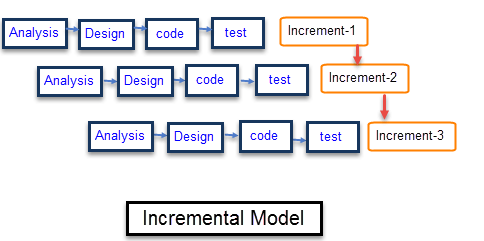
\includegraphics[width=0.9\textwidth]{figs/modelo_incremental.png}
    \caption{Representación del modelo incremental.}
    \label{fig:modelo-incremental}
\end{figure}

\section{Planificaci\'on temporal}
\subsection{Descomposición de tareas por fases}
La planificación se ha dividido en siete bloques principales: \textbf{Inicio, Estado del arte, An\'alisis, Dise\~no, Implementaci\'on, Pruebas} y \textbf{Documentaci\'on}, en concordancia con el modelo incremental utilizado.

\subsubsection*{1. Inicio}
\begin{itemize}
  \item Estudio del problema que resuelve la app
  \item Definición de objetivos del TFG
  \item Planificación inicial del proyecto
\end{itemize}

\subsubsection*{2. Estado del arte}
\begin{itemize}
  \item Revisión de apps similares educativas, con RA y mapas
  \item Estudio de mujeres y sus lugares en Valencia
  \item Estudio de frameworks de RA, mapas y escáneres QR
  \item Selección de tecnologías definitivas (React Native, Django, AFrame)
\end{itemize}

\subsubsection*{3. Análisis}
\begin{itemize}
  \item Definición detallada de requisitos funcionales y no funcionales
  \item Modelado inicial del sistema: navegación y casos de uso
  \item Modelado entidad-relación de la base de datos
  \item Definición de métricas y rutas
\end{itemize}

\subsubsection*{4. Diseño}
\begin{itemize}
  \item Diseño de la arquitectura frontend y backend
  \item Diseño de interfaz móvil y estilo visual
  \item Diseño de pantallas clave: login, listado, mapa, RA, etc.
\end{itemize}

\subsubsection*{5. Implementación backend}
\begin{itemize}
  \item Creación del proyecto Django y configuración Docker
  \item Creación de modelos de datos y migraciones
  \item Implementación de API REST para usuarios, lugares y rutas
  \item Sistema de login y sesiones
  \item Registro de visitas, logros y progreso
\end{itemize}

\subsubsection*{6. Implementación frontend}
\begin{itemize}
  \item Configuración base y navegación
  \item Registro e inicio de sesión de usuarios
  \item Implementación del listado y filtros por ámbito y visitas
  \item Implementación del historial de usuario
  \item Implementación de mapa con geolocalización
  \item Escaneo de QR y navegación a detalle
  \item Sincronización de datos con backend
\end{itemize}

\subsubsection*{7. Implementación de realidad aumentada}
\begin{itemize}
  \item Configuración de AR.js y marcador personalizado
  \item Activación de RA según la ubicación (menos de 1km)
  \item Visualización de modelo 3D y contenido RA educativo
\end{itemize}

\subsubsection*{8. Pruebas y validación}
\begin{itemize}
  \item Pruebas funcionales de cada módulo
  \item Pruebas completas con usuarios externos
  \item Corrección de errores y mejoras detectadas
\end{itemize}

\subsubsection*{9. Documentación}
\begin{itemize}
  \item Redacción progresiva de la memoria (paralela a todo el desarrollo)
  \item Revisión completa, maquetación y anexos finales
\end{itemize}

\subsection{Estimación temporal}
La técnica de estimación utilizada es la media beta de probabilidad. Para cada tarea se ha asignado un tiempo optimista (TO), pesimista (TP) y más probable (TM), y se ha calculado la duración estimada (TE) con la siguiente fórmula:

\begin{center}
$TE = \frac{TO + 4 \cdot TM + TP}{6}$
\end{center}

\begin{table}[H]
\centering
\caption{Estimación por tres valores de las tareas del proyecto}
\begin{tabular}{|l|c|c|c|c|}
\hline
\textbf{Tarea} & \textbf{TO} & \textbf{TP} & \textbf{TM} & \textbf{TE} \\
\hline
Estudio del problema & 1 & 3 & 2 & 2.00 \\
Definición de objetivos & 1 & 2 & 1 & 1.17 \\
Planificación inicial & 1 & 2 & 1 & 1.17 \\
Revisión apps similares & 2 & 4 & 3 & 3.00 \\
Estudio lugares mujeres & 1 & 3 & 2 & 2.00 \\
Frameworks RA y QR & 2 & 4 & 3 & 3.00 \\
Selección tecnologías & 1 & 2 & 1 & 1.17 \\
Requisitos funcionales & 2 & 4 & 3 & 3.00 \\
Casos de uso y navegación & 1 & 3 & 2 & 2.00 \\
Modelo E-R BD & 1 & 3 & 2 & 2.00 \\
Def. métricas y rutas & 1 & 2 & 1 & 1.17 \\
Diseño arquitectura & 2 & 4 & 3 & 3.00 \\
Diseño interfaz visual & 2 & 5 & 3 & 3.17 \\
Pantallas clave & 2 & 4 & 3 & 3.00 \\
Django y Docker & 1 & 3 & 2 & 2.00 \\
Modelos y migraciones & 1 & 3 & 2 & 2.00 \\
API usuarios y lugares & 3 & 5 & 4 & 4.00 \\
Login y sesiones & 1 & 3 & 2 & 2.00 \\
Registro visitas y logros & 1 & 3 & 2 & 2.00 \\
Conf. navegación base & 1 & 3 & 2 & 2.00 \\
Registro e inicio sesión & 1 & 3 & 2 & 2.00 \\
Listado y filtros & 2 & 4 & 3 & 3.00 \\
Historial de usuario & 1 & 3 & 2 & 2.00 \\
Mapa geolocalizado & 2 & 4 & 3 & 3.00 \\
Escaneo QR & 1 & 3 & 2 & 2.00 \\
Sincronización datos & 1 & 3 & 2 & 2.00 \\
Config. AR.js y marcador & 1 & 3 & 2 & 2.00 \\
Desbloqueo por distancia & 1 & 3 & 2 & 2.00 \\
Visualización RA & 2 & 4 & 3 & 3.00 \\
Pruebas funcionales & 2 & 4 & 3 & 3.00 \\
Pruebas con usuarios & 1 & 3 & 2 & 2.00 \\
Corrección errores & 1 & 3 & 2 & 2.00 \\
Redacción progresiva & 4 & 6 & 5 & 5.00 \\
Revisión y entrega final & 2 & 4 & 3 & 3.00 \\
\hline
\textbf{Total estimado} & 73 & 127 & 96 & \textbf{100.00 días} \\
\hline
\end{tabular}
\end{table}

\subsection{Diagrama de Gantt}

Para representar la planificación temporal del proyecto de forma visual, se ha elaborado un diagrama de Gantt utilizando \texttt{Microsoft Project}, teniendo en cuenta las dependencias y la posibilidad de solapar tareas como la documentación progresiva.

\begin{figure}[H]
    \centering
    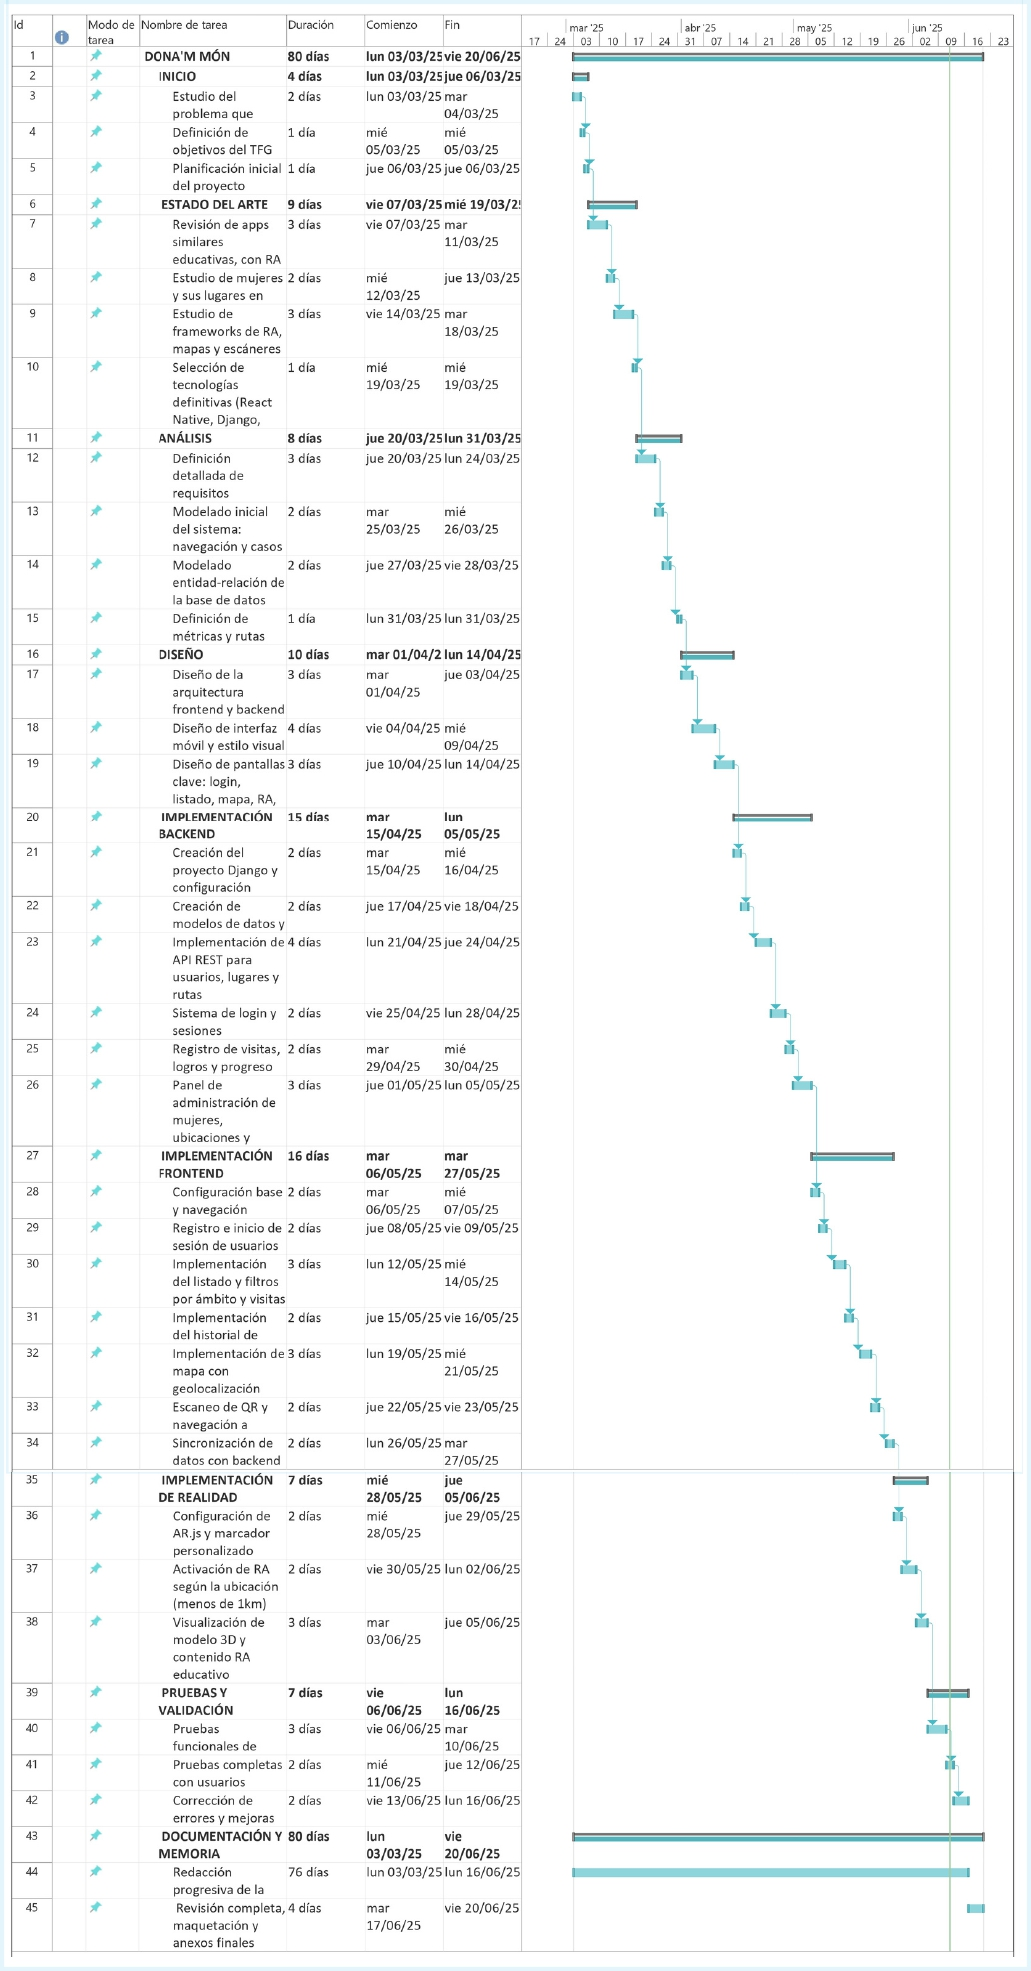
\includegraphics[width=\textwidth,height=0.95\textheight,keepaspectratio]{figs/gantt.jpg}
    \caption{Diagrama de Gantt detallado del proyecto.}
    \label{fig:gantt}
\end{figure} 

A pesar de que la estimación por tres valores del proyecto arroja una duración total de aproximadamente \textbf{100 días} (equivalente a \textbf{800 horas}), el desarrollo real se ha planificado a lo largo de \textbf{80 días laborables} (como puede observarse en el diagrama de Gantt), lo que supone un total de \textbf{640 horas efectivas} de trabajo, distribuidas en jornadas de \textbf{8 horas al día}.

Cabe destacar que:
\begin{itemize}
    \item El proyecto se ha realizado en paralelo con el \textit{Máster en Tecnologías Web, Computación en la Nube y Aplicaciones Móviles}.
    \item Además, durante este periodo se estaban llevando a cabo \textit{prácticas extracurriculares en el Instituto de Robótica y Tecnologías de la Información y la Comunicación (IRTIC)}, donde también se ha avanzado el desarrollo del TFG.
    \item No se ha trabajado durante los fines de semana, por lo que los 80 días corresponden exclusivamente a días laborables.
\end{itemize}

La fecha de inicio del proyecto fue el \textbf{3 de marzo de 2025}, y la fecha de finalización fue el \textbf{20 de junio de 2025}. El proyecto ha sido planificado y ejecutado con el objetivo de ser presentado en la \textbf{primera convocatoria}.
\section{Estimación de costes}

La estimación económica del proyecto se ha realizado distinguiendo entre:
\begin{itemize}
  \item \textbf{Costes directos de personal:} incluyen el salario bruto anual para cada perfil profesional, junto con los costes de Seguridad Social correspondientes (aproximadamente un 30\% adicionales). Se han considerado perfiles distintos (Jefe de Proyecto, Desarrollador Backend, Desarrollador Frontend, Desarrolador de Realidad Tester/QA y Modelador 3D), aunque el proyecto sea llevado a cabo por una sola persona.
  \item \textbf{Costes directos de material:} contemplan licencias, equipos y amortización del hardware y software utilizado.
  \item \textbf{Costes indirectos:} coeficiente adicional del 20\% aplicado sobre el total de los costes directos, para cubrir gastos generales asociados (electricidad, internet, etc.).
\end{itemize}


Este desglose permite dimensionar correctamente los recursos implicados y simular una estructura empresarial.

\subsection{Costes directos de personal}

Se han obtenido los sueldos medios anuales en España para cada perfil profesional a partir del portal \textit{Glassdoor}~\cite{glassdoorJefeProyecto,glassdoorFrontend,glassdoorBackend,glassdoorTester,glassdoorModelador3D,glassdoorDiseñadr,glassdoorARDeveloper}. A cada salario bruto se le añade un 30\% adicional correspondiente a cotizaciones sociales: contingencias comunes, desempleo, formación y Fogasa.

Se asume una jornada laboral de 8~h/día, 20 días laborables por mes y 11 meses de trabajo al año, siendo 220 días laborales al año. La planificación se basa en 80 días efectivos de trabajo entre el \textbf{3 de marzo y el 20 de junio de 2025}, distribuidos entre los distintos perfiles según su implicación en cada fase.

\begin{table}[H]
\centering
\caption{Perfiles y costes de personal (según cotización SS 2025)}
\begin{tabular}{|l|r|r|r|r|r|}
\hline
\textbf{Perfil} & \textbf{Bruto/año (€)} & \textbf{+31.4\% SS (€)} & \textbf{Total (€)} & \textbf{€/día} & \textbf{€/h} \\
\hline
Jefe de Proyecto        & 40\,500 & 12\,717.00 & 53\,217.00 & 270.92 & 33.87 \\
Desarrollador Frontend  & 40\,500 & 12\,717.00 & 53\,217.00 & 270.92 & 33.87 \\
Desarrollador Backend   & 30\,000 & 9\,420.00  & 39\,420.00 & 200.10 & 25.01 \\
Desarrollador RA        & 23\,000 & 7\,222.00  & 30\,222.00 & 153.68 & 19.21 \\
Tester / QA             & 23\,500 & 7\,379.00  & 30\,879.00 & 156.71 & 19.59 \\
Modelador 3D            & 12\,000 & 3\,768.00  & 15\,768.00 & 79.84  & 9.98  \\
Diseñador gráfico       & 26\,000 & 8\,164.00  & 34\,164.00 & 173.32 & 21.67 \\
\hline
\end{tabular}
\end{table}



\subsection{Asignación temporal por perfil}

Se ha asignado a cada perfil el número estimado de jornadas necesarias para cubrir las tareas planificadas según el cronograma de trabajo. A continuación, se presenta la estimación de coste directo de personal en función de esas jornadas.

\begin{table}[H]
\centering
\caption{Asignación de tareas y costes por perfil}
\begin{tabular}{|l|c|r|p{6.5cm}|r|}
\hline
\textbf{Perfil} & \textbf{Días} & \textbf{€/día} & \textbf{Tareas} & \textbf{Coste (€)} \\
\hline
Jefe de Proyecto & 50 & 270.92 & Estudio inicial, definición de objetivos, planificación, selección de tecnologías, coordinación general & 13,546.00 \\
\hline
Desarrollador Frontend & 16 & 270.92 & Diseño arquitectura frontend, desarrollo UI, navegación, QR, filtros, mapa & 4,334.72 \\
\hline
Desarrollador Backend & 15 & 200.10 & Creación API Django, modelo de datos, autenticación, sincronización backend & 3,001.50 \\
\hline
Desarrollador RA & 7 & 153.68 & Integración AR.js, activación por proximidad, carga de modelos RA & 1,075.76 \\
\hline
Tester / QA & 7 & 156.71 & Pruebas funcionales, pruebas con usuarios, validación y corrección de errores & 1,096.97 \\
\hline
Modelador 3D & 15 & 79.84 & Diseño y preparación de modelos 3D para RA & 1,197.60 \\
\hline
Diseñador gráfico & 20 & 173.32 & Diseño interfaz, estilo visual, iconos y logotipos & 3,466.40 \\
\hline
\end{tabular}
\end{table}

\subsection{Costes directos de material}

Los costes directos de material comprenden los recursos físicos y licencias digitales utilizados durante el desarrollo del proyecto. Para estimar su impacto económico real, se ha calculado la amortización proporcional al tiempo de uso, aplicando la fórmula:

\[
\text{Amortización} = \frac{\text{Precio unidad} \times \text{Días de uso}}{\text{Días de vida útil}}
\]

\begin{table}[H]
\centering
\small
\caption{Elementos utilizados y coste amortizado durante el desarrollo (80 días)}
\resizebox{0.92\textwidth}{!}{%
\begin{tabular}{|l|r|c|c|r|}
\hline
\textbf{Elemento} & \textbf{Precio (€)} & \textbf{Vida útil} & \textbf{Uso (días)} & \textbf{Coste amortizado (€)} \\
\hline
Portátil Asus ROG Strix G15      & 999.00 & 5 años (1825 días)  & 80 & 43.79 \\
iPhone 11                        & 749.00 & 4 años (1460 días)  & 80 & 41.03 \\
Ratón Logitech G203              & 20.99  & 5 años (1825 días)  & 80 & 0.92  \\
Visual Paradigm (mensual)        & 30.00  & 30 días              & 30 & 30.00 \\
Microsoft 365 Business Standard  & 12.50  & 30 días              & 30 & 12.50 \\
Visual Studio Code (profesional) & 45.00  & 365 días             & 80 & 9.86  \\
Docker Pro                       & 99.00  & 365 días             & 80 & 21.70 \\
GitHub Copilot                   & 100.00 & 365 días             & 80 & 21.92 \\
Overleaf Premium                 & 140.00 & 365 días             & 80 & 30.68 \\
\hline
\multicolumn{4}{|r|}{\textbf{Total amortizado}} & \textbf{212.40 €} \\
\hline
\end{tabular}
}%
\end{table}


Cabe destacar que varias de estas herramientas (como Visual Studio Code, Docker o GitHub) disponen de versiones gratuitas o de acceso académico, pero se ha optado por reflejar el coste real de uso profesional para una estimación más realista.

\subsection{Costes indirectos}

Los costes indirectos se han estimado aplicando un coeficiente adicional del 20\% sobre el total de los costes directos (personal y material). Este porcentaje se considera representativo para cubrir gastos generales como el consumo eléctrico, conexión a internet, mantenimiento del equipo, uso de espacios compartidos y otros recursos no imputables directamente al desarrollo del proyecto, pero imprescindibles para su ejecución.

\[
\text{Costes indirectos} = (\text{Costes directos de personal} + \text{Costes directos de material}) \times 0.20
\]

\[
\text{Costes indirectos} = (27\,718.95\ € + 212.40\ €) \times 0.20 = 5\,586.27\ €
\]

\subsection{Coste total del proyecto}

A partir de la suma de los distintos componentes estimados (personal, material e indirectos), se obtiene el coste total simulado del desarrollo del proyecto en un entorno profesional.

\begin{table}[H]
\centering
\caption{Resumen de costes del proyecto}
\begin{tabular}{|l|r|}
\hline
\textbf{Concepto} & \textbf{Coste (€)} \\
\hline
Costes directos de personal & 27\,718.95 \\
Costes directos de material & 212.40 \\
Costes indirectos (20\%) & 5\,586.27 \\
\hline
\textbf{Coste total estimado} & \textbf{33\,517.62} \\
\hline
\end{tabular}
\end{table}

Esta estimación permite cuantificar de forma realista los recursos necesarios para ejecutar un proyecto de características similares en un entorno empresarial. Aunque el trabajo haya sido desarrollado por una única persona, se ha optado por realizar una simulación profesional con perfiles especializados para reflejar adecuadamente la complejidad técnica y el valor añadido del producto final.

\section{Viabilidad del proyecto}

\subsection{Viabilidad económica}

El análisis de costes realizado en la sección anterior ha permitido cuantificar los recursos necesarios para el desarrollo de la aplicación \textit{DONA’m MÓN}. El coste total estimado, que incluye los costes directos de personal (27.718,95~€), costes directos de material (212,40~€) y un 20\% adicional en concepto de costes indirectos (5.586,27~€), asciende a \textbf{33.517,62~€}.

Dado que el proyecto se ha desarrollado sin fines comerciales, el desarrollo ha sido ejecutado por una única persona, utilizando licencias gratuitas, versiones académicas o software de código abierto. Por tanto, los costes no se han asumido en su totalidad. No obstante, se ha realizado una estimación económica completa con el objetivo de evaluar su viabilidad en un contexto profesional o empresarial real, permitiendo así dimensionar correctamente los recursos necesarios en caso de una futura implementación a escala.

El presupuesto puede considerarse razonable si se contempla una posible financiación pública (subvenciones a proyectos culturales, feministas o tecnológicos), financiación universitaria, patrocinio institucional (ayuntamientos, universidades o fundaciones), o apoyo por parte de entidades interesadas en promover la visibilización de mujeres en entornos urbanos y educativos. Además, el impacto social y educativo del proyecto puede justificar su financiación mediante convocatorias de innovación social o género.

\subsection{Viabilidad legal}

Desde el punto de vista legal, el desarrollo de esta aplicación requiere considerar varias cuestiones relevantes:

\begin{itemize}
\item \textbf{Protección de datos personales (RGPD)}: la aplicación permite el registro de usuarios y almacena información relacionada con su ubicación geográfica y su historial de visitas. Por ello, se deberá garantizar el cumplimiento del Reglamento General de Protección de Datos (RGPD), asegurando la obtención del consentimiento explícito del usuario, el almacenamiento seguro de datos y la posibilidad de acceder, rectificar o eliminar la información personal.
\item \textbf{Política de privacidad y condiciones de uso}: será necesario incluir una política clara y accesible que informe al usuario sobre el tratamiento de sus datos, el uso de la geolocalización y la finalidad educativa de la aplicación.

\item \textbf{Derechos de autor y licencias}: todos los modelos 3D, imágenes, textos y recursos utilizados deben contar con licencia libre (Creative Commons, dominio público) o haber sido creados expresamente para el proyecto. En caso contrario, sería necesario solicitar los permisos adecuados.

\item \textbf{Política de uso de servicios externos}: la aplicación hace uso de tecnologías como \textit{WebView} para integrar experiencias de realidad aumentada desarrolladas con A-Frame y AR.js, por lo que se han respetado sus licencias de uso (ambas de código abierto bajo licencia MIT), garantizando la legalidad del uso de estas herramientas dentro del proyecto.
\end{itemize}

No se han identificado restricciones legales insalvables que impidan la realización o publicación de la aplicación. En todo caso, se recomienda aplicar buenas prácticas en el desarrollo seguro, accesible y ético del software.
\section{Análisis de riesgos}

Durante el desarrollo del proyecto \textit{DONA'm MÓN} se han identificado diversos riesgos que pueden afectar negativamente a su cumplimiento en tiempo, coste o calidad. Para su evaluación se ha utilizado un enfoque cualitativo que combina la estimación de la probabilidad de ocurrencia y el impacto en el proyecto, permitiendo establecer niveles de riesgo y su clasificación prioritaria.

\subsection{Principales riesgos identificados}

En la Tabla~\ref{tabla:riesgos-identificados} se recogen los principales riesgos detectados, su probabilidad estimada, el impacto medido en días de retraso potencial, su nivel de riesgo (NR = Probabilidad × Impacto), la clasificación resultante y la fase del proyecto en la que podrían manifestarse.

\begin{table}[H]
\centering
\caption{Principales riesgos identificados}
\label{tabla:riesgos-identificados}
\resizebox{\textwidth}{!}{%
\begin{tabular}{|p{5cm}|c|c|c|c|c|}
\hline
\textbf{Riesgo} & \textbf{Prob. (\%)} & \textbf{Impacto (días)} & \textbf{NR} & \textbf{Clasificación} & \textbf{Fase} \\
\hline
Retrasos en la integración de la RA con React Native & 40 & 8 & 3.20 & Inaceptable & Ejecución \\
Cambios en dependencias externas (Mapas, RA, etc.) & 30 & 5 & 1.50 & Alto & Ejecución \\
Falta de experiencia previa con tecnologías clave & 35 & 6 & 2.10 & Alto & Planificación/Ejecución \\
Definición ambigua del alcance inicial & 25 & 7 & 1.75 & Alto & Inicio \\
Estimaciones optimistas en tareas críticas & 20 & 6 & 1.20 & Moderado & Planificación \\
Problemas legales (datos, localización, RGPD) & 15 & 5 & 0.75 & Moderado & Inicio \\
Baja disponibilidad de recursos y tiempo personal & 30 & 6 & 1.80 & Alto & Ejecución \\
Errores funcionales en fases finales & 10 & 5 & 0.50 & Bajo & Cierre \\
\hline
\end{tabular}
}
\end{table}


A continuación se describen los riesgos con mayor nivel de prioridad:

\begin{enumerate}
  \item \textbf{Definición ambigua del alcance del proyecto:} Un alcance mal delimitado puede derivar en objetivos poco claros y decisiones incorrectas en fases posteriores del desarrollo.

  \textit{Probabilidad: Media — Impacto: Alto — Nivel de riesgo: Inaceptable}

  \item \textbf{Estimaciones temporales y de costes imprecisas:} Una planificación optimista puede provocar desviaciones significativas respecto al cronograma o sobrecostes imprevistos.

  \textit{Probabilidad: Alta — Impacto: Alto — Nivel de riesgo: Inaceptable}

  \item \textbf{Falta de experiencia con tecnologías específicas:} La falta de familiaridad con herramientas clave como AR.js o A-Frame podría ralentizar la implementación de la funcionalidad de realidad aumentada.

  \textit{Probabilidad: Media — Impacto: Alto — Nivel de riesgo: Inaceptable}

  \item \textbf{Retrasos en la ejecución de tareas clave:} La elevada carga de trabajo asumida por una sola persona incrementa la probabilidad de bloqueos o demoras.

  \textit{Probabilidad: Alta — Impacto: Medio — Nivel de riesgo: Alto}

  \item \textbf{Dependencia de recursos externos:} El uso de librerías de terceros (como AR.js, Mapbox, A-Frame) puede verse afectado por cambios inesperados o falta de mantenimiento.

  \textit{Probabilidad: Media — Impacto: Medio — Nivel de riesgo: Medio}

  \item \textbf{Problemas de compatibilidad entre componentes:} La integración entre tecnologías heterogéneas (React Native, Django, AR.js) podría causar errores o conflictos difíciles de prever.

  \textit{Probabilidad: Baja — Impacto: Alto — Nivel de riesgo: Alto}

  \item \textbf{Riesgos legales:} A pesar de que no se almacena información sensible, el tratamiento de datos de geolocalización y el uso de usuarios registrados exige el cumplimiento de la normativa vigente en materia de protección de datos (RGPD).

  \textit{Probabilidad: Baja — Impacto: Medio — Nivel de riesgo: Medio}
\end{enumerate}


\subsection{Matriz de riesgos}

La figura~\ref{fig:matriz-riesgos} muestra la matriz de evaluación de riesgos utilizada, que relaciona la probabilidad de ocurrencia con la magnitud del impacto. Esta herramienta facilita la clasificación de los riesgos y la priorización de acciones preventivas.

\begin{figure}[H]
\centering
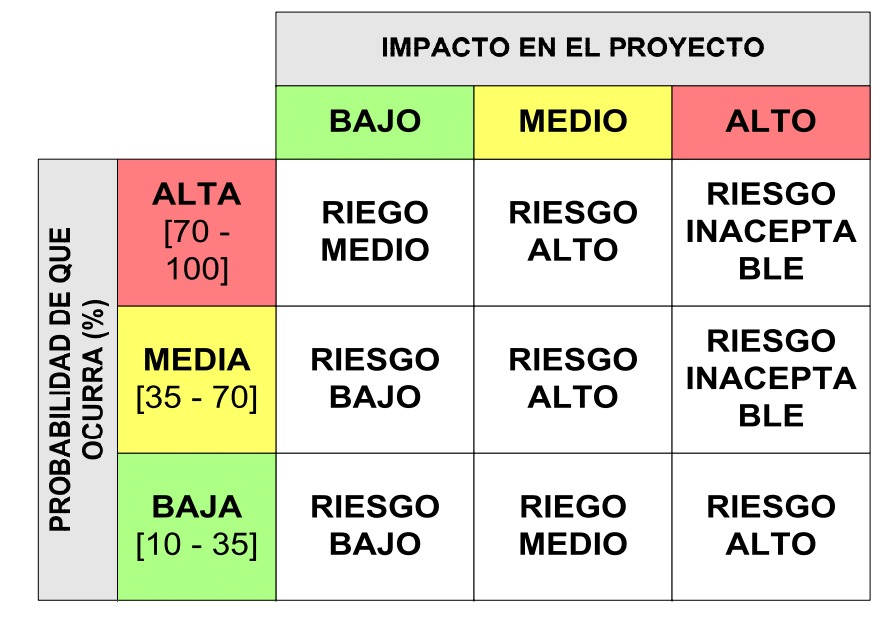
\includegraphics[width=0.65\textwidth]{matriz_riesgos.jpg}
\caption{Matriz de priorización de riesgos utilizada}
\label{fig:matriz-riesgos}
\end{figure}

\subsection{Resumen de evaluación de riesgos}

\begin{table}[H]
\centering
\caption{Resumen cualitativo de evaluación de riesgos}
\label{tabla:resumen-riesgos}
\begin{tabular}{|p{5.5cm}|c|c|c|}
\hline
\textbf{Riesgo} & \textbf{Probabilidad} & \textbf{Impacto} & \textbf{Clasificación} \\
\hline
Definición ambigua del alcance & Media & Alto & Inaceptable \\
Estimaciones temporales imprecisas & Alta & Alto & Inaceptable \\
Falta de experiencia con RA & Media & Alto & Inaceptable \\
Retrasos en tareas clave & Alta & Medio & Alto \\
Dependencia de recursos externos & Media & Medio & Medio \\
Problemas de compatibilidad tecnológica & Baja & Alto & Alto \\
Riesgos legales (RGPD) & Baja & Medio & Medio \\
\hline
\end{tabular}
\end{table}

\subsection{Estrategias de mitigación}

Para minimizar el impacto de los riesgos identificados en el proyecto, se han definido una serie de medidas preventivas orientadas a reducir su probabilidad de ocurrencia o su impacto en caso de materializarse. Estas estrategias se alinean con las buenas prácticas en la gestión de proyectos tecnológicos y tienen carácter proactivo.

\begin{itemize}
  \item \textbf{Definición ambigua del alcance del proyecto:} Se ha trabajado desde el inicio con una delimitación clara del alcance y los objetivos, apoyada por una estructura modular de tareas y entregables. La revisión periódica del cronograma y del backlog funcional permite detectar desviaciones tempranas y corregir posibles ambigüedades.

  \item \textbf{Estimaciones temporales y de costes imprecisas:} La planificación se ha fundamentado en la técnica de estimación por tres valores (optimista, más probable y pesimista), reduciendo la subjetividad y permitiendo incorporar márgenes de seguridad en tareas críticas. Además, se han utilizado referencias de proyectos similares como guía de validación.

  \item \textbf{Falta de experiencia con tecnologías específicas:} Durante la fase de análisis técnico se han realizado pruebas de concepto con las tecnologías clave (AR.js, A-Frame, integración con React Native) para identificar dificultades de forma anticipada. Asimismo, se ha recurrido a documentación oficial, foros especializados y comunidades activas.

  \item \textbf{Retrasos en la ejecución de tareas clave:} Dado que el proyecto es desarrollado por una única persona, se han asignado holguras temporales en tareas críticas y puntos de control semanales para verificar el avance real. El uso de herramientas como Microsoft Project ha permitido detectar desviaciones y replanificar en tiempo real.

  \item \textbf{Dependencia de recursos externos:} Se ha priorizado el uso de herramientas open source con comunidades activas y mantenidas (por ejemplo, AR.js, OpenStreetMap). Además, se han definido posibles alternativas ante fallos o incompatibilidades en recursos externos.

  \item \textbf{Problemas de compatibilidad entre componentes:} La arquitectura del sistema se ha diseñado de forma desacoplada, favoreciendo la integración por medio de interfaces RESTful y estándares abiertos. Esto reduce la posibilidad de conflictos entre tecnologías heterogéneas.

  \item \textbf{Riesgos legales (RGPD):} Aunque no se almacenan datos sensibles, se garantiza el cumplimiento normativo mediante el uso de comunicaciones seguras (HTTPS), el consentimiento del usuario para acceder a la ubicación y la ausencia de almacenamiento persistente de información personal.
\end{itemize}


\subsection{Planes de contingencia}

Se han previsto planes de contingencia específicos para los riesgos más relevantes. Por ejemplo, si se detectan incompatibilidades graves entre tecnologías, se contemplaría el uso de una solución alternativa basada únicamente en mapas interactivos sin RA, manteniendo la funcionalidad básica de exploración de contenidos educativos geolocalizados.

